\chapter{Validación}

\section{Metodología de validación}

Para validar la eficacia del modelo de detección de anomalías en subespacios, se propone una metodología que evalúa sus resultados desde dos dimensiones complementarias: una cualitativa, orientada a la utilidad clínica de las alertas generadas, y otra cuantitativa, enfocada en la relación entre el indicador de criticidad desarrollado y el estado real del paciente medido a través de sus signos vitales.

Primero, a nivel cualitativo se examinan las alertas generadas por el modelo de subespacios para determinar si proporcionan información útil, relevante y accionable para los profesionales de la salud. En este análisis se comparan las alertas de nuestro modelo con las alertas producidas por el modelo previo empleado sobre el mismo paciente en idénticos intervalos de tiempo. Para ello, se revisan las alertas identificadas por cada sistema y se evalúa si las nuevas alertas permiten: (1) anticipar de manera oportuna eventos de deterioro clínico, (2) ofrecer indicaciones claras sobre qué parámetro o combinación de parámetros está fuera de lo esperado y (3) orientar la toma de decisiones médicas de forma más precisa.

En segundo lugar, el análisis cuantitativo busca demostrar que las anomalías reportadas efectivamente coinciden con los momentos en los que el paciente experimenta mayor criticidad fisiológica. Para ello, se utiliza como referencia el número de signos vitales que, en un instante dado, se encuentran fuera de sus rangos normales definidos para la población pediátrica en la UCIP. Este conteo de parámetros alterados se registra segundo a segundo y se considera una medida objetivo para definir el estado del paciente. La Figura \ref{fig:patient3_signos_vitales_fuera_de_rango}, presenta el resultado de calcular el numero de signos vitales fuera de rango en cada instante de tiempo para el paciente 3.

Para facilitar la comparación, este número de signos vitales fuera de rango se clasifica nuevamente en tres categorías de riesgo: alto, medio y bajo. La clasificación se realiza de la siguiente manera: se considera alto riesgo cuando más de dos tercios de los signos vitales monitorizados en ese instante se encuentran fuera de los límites normales; riesgo medio si la proporción de signos vitales alterados está entre un tercio y dos tercios; y bajo riesgo cuando un tercio o menos de los signos vitales presentan valores fuera del rango normal para la edad del paciente. Este criterio es consistente con la metodología utilizada previamente para determinar el nivel de alerta a partir del indicador de criticidad, asegurando así coherencia en la evaluación.

\begin{figure}[H]
  \centering
  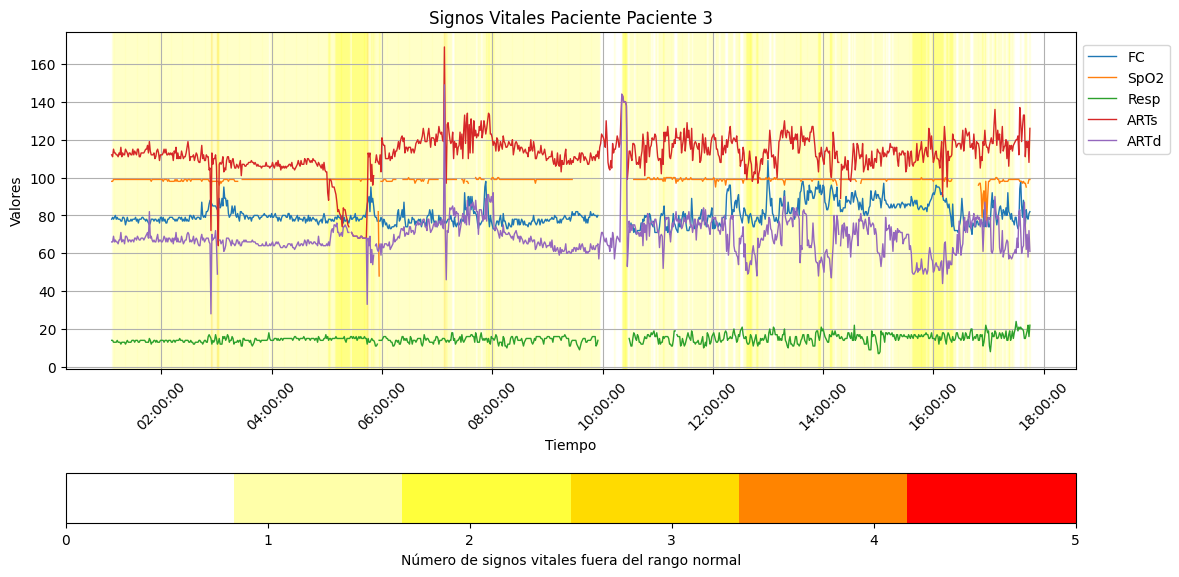
\includegraphics[width=\textwidth]{Images/patient3_signos_vitales_fuera_de_rango_2.png}
  \caption{Número de signos vitales fuera de rango para el paciente 3.}
  \label{fig:patient3_signos_vitales_fuera_de_rango}
\end{figure}

A partir de esta categorización, se determina si el modelo clasificó correctamente el estado del paciente en los diferentes instantes de tiempo, comparando la categoría de riesgo asignada por el modelo con la obtenida a partir de los signos vitales reales. Esto permite calificar la exactitud y precisión de los resultados del modelo, evaluando su capacidad para discriminar entre situaciones de mayor y menor criticidad fisiológica.A continuación, se presentan los rangos de normalidad de los signos vitales para cada grupo etario, que se utilizarán como referencia para la validación del modelo.

\begin{table}[H]
  \centering
  \resizebox{\textwidth}{!}{%
    \begin{tabular}{lccccc}
      \rowcolor[HTML]{AFB8CC}
      \textbf{Signo Vital} & \textbf{0-1 años} & \textbf{1-3 años} & \textbf{4-5 años} & \textbf{6-12 años} & \textbf{13-18 años} \\
      \rowcolor[HTML]{E8E8E8}
      ARTs (mmHg) & 60--90 & 78--112 & 85--114 & 95--135 & 100--120 \\
      ARTd (mmHg) & 30--62 & 48--78 & 52--85 & 58--88 & 60--80 \\
      FC (lpm)    & 100--160 & 95--150 & 80--140 & 70--120 & 60--100 \\
      Resp (rpm)  & 30--60 & 24--40 & 22--34 & 18--30 & 12--16 \\
      SpO$_2$ (\%) & 88--100 & 88--100 & 88--100 & 88--100 & 88--100 \\
    \end{tabular}%
  }
  \caption{Rangos normales de signos vitales según grupo etario. ARTs: Presión arterial sistólica; ARTd: Presión arterial diastólica; FC: Frecuencia cardíaca; Resp: Frecuencia respiratoria; SpO$_2$: Saturación de oxígeno.}
  \label{tab:rangos_signos_vitales}
\end{table}

\section{Resultados}

Los resultados de la validación del modelo de detección de anomalías en subespacios se presentan a continuación, organizados en dos secciones: una que resume los hallazgos cualitativos y otra que detalla los resultados cuantitativos obtenidos.

\subsection{Resultados cuantitativos}

En esta sección se presentan los resultados cuantitativos de la validación del modelo de detección de anomalías en subespacios. El objetivo principal es comparar la clasificación del estado de criticidad del paciente realizada por el indicador propuesto frente a la clasificación basada en el número de signos vitales fuera de rango, considerada como referencia objetiva. Esta comparación permite evaluar la capacidad del modelo para identificar correctamente los periodos de mayor riesgo fisiológico, y reportar alertas que sean coherentes con el estado real del paciente.

Para ilustrar esta comparación, la Figura \ref{fig:comparacion_clasificacion_paciente3} muestra, para el paciente 3, la evolución temporal de cual es el nivel de alerta asignada por el indicador de criticidad y la categoría obtenida a partir del conteo de signos vitales fuera de rango. En el diagrama, cada instante de tiempo se clasifica como riesgo bajo, medio o alto según ambos métodos, permitiendo visualizar la concordancia y las discrepancias entre ellos.

\begin{figure}[H]
  \centering
  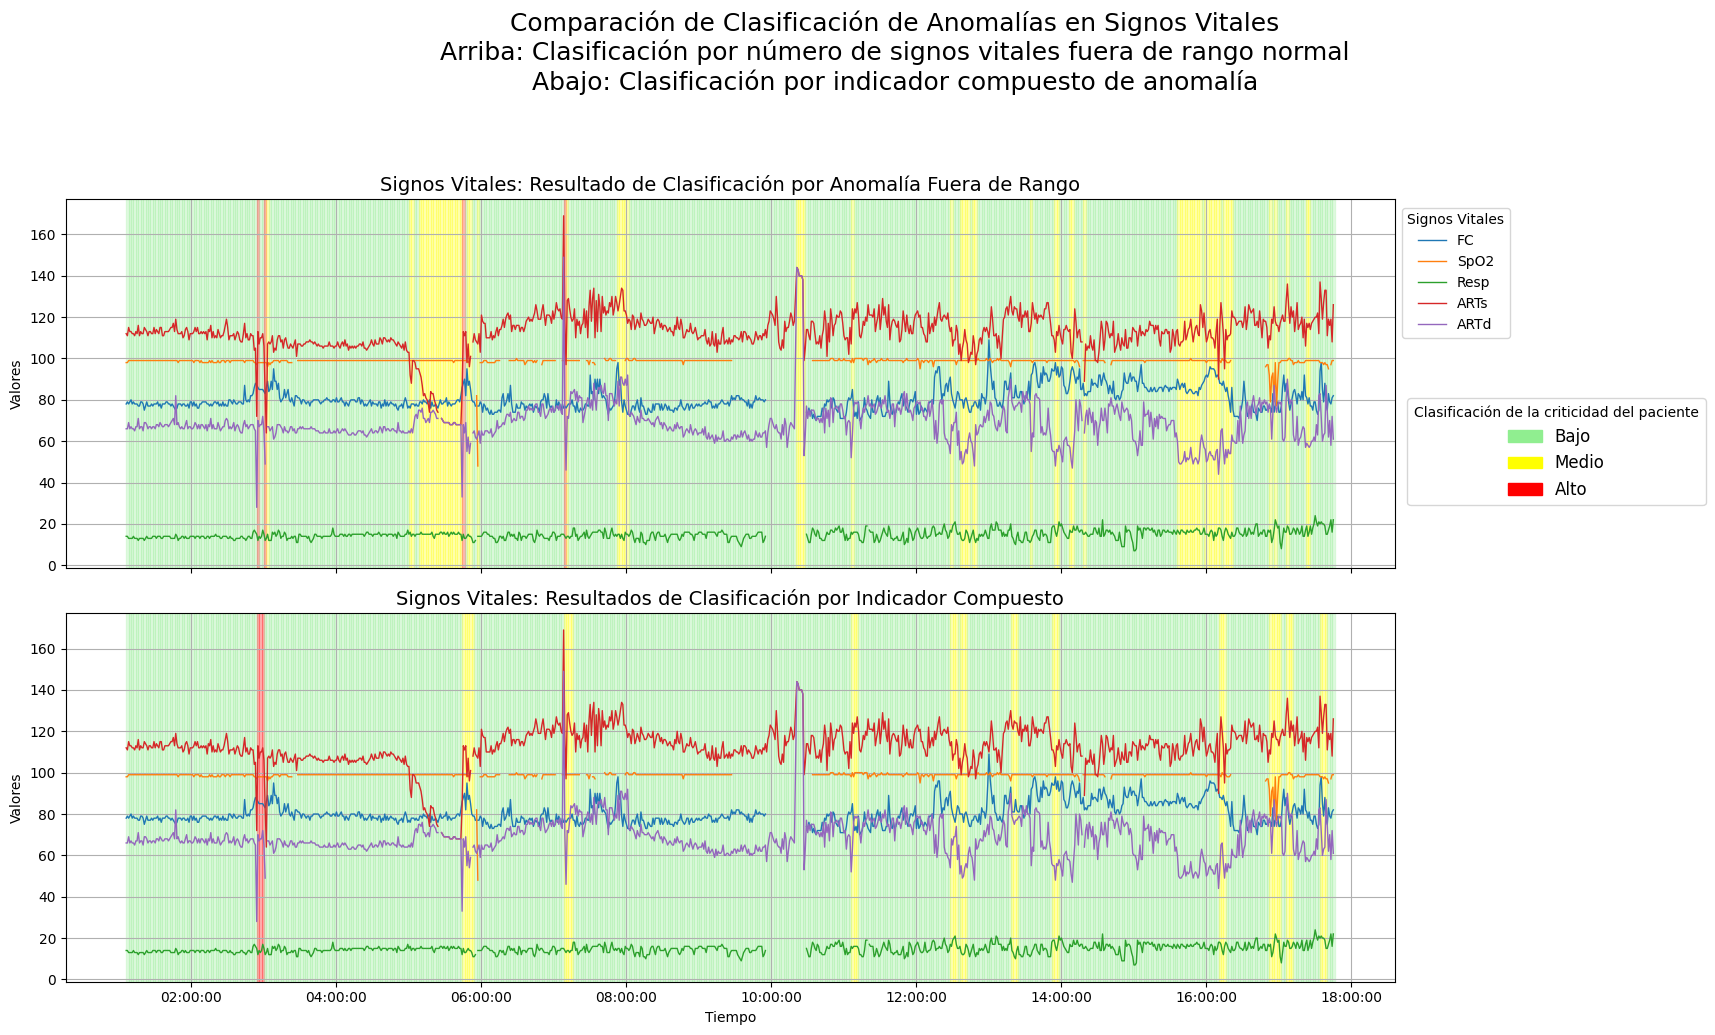
\includegraphics[width=\textwidth]{Images/comparacion_indicador_con_fuera_de_rango.png}
  \caption{Comparación de la clasificación de criticidad para el paciente 3: indicador de criticidad vs. número de signos vitales fuera de rango.}
  \label{fig:comparacion_clasificacion_paciente3}
\end{figure}

A partir de esta comparación, se observa que el indicador de criticidad propuesto logra identificar correctamente los periodos de alto riesgo fisiológico en la mayoría de los casos, coincidiendo con los momentos donde la mayoría de los signos vitales se encuentran por fuera del rango normal. Además, el modelo muestra una buena capacidad para discriminar entre situaciones de riesgo medio y bajo, reflejando adecuadamente las fluctuaciones en el estado del paciente a lo largo del tiempo.

A continuación, la Tabla \ref{tab:resultados_cuantitativos} resume los resultados cuantitativos obtenidos para todos los pacientes incluidos en la validación. En este contexto, la precisión se refiere a la proporción de instantes en los que el indicador de criticidad predicho por el modelo coincide exactamente con la categoría de riesgo determinada a partir del número de signos vitales fuera de rango. Es decir, mide qué tan confiables son las alertas generadas por el modelo: de todas las veces que el modelo indicó un cierto nivel de riesgo, cuántas veces esa alerta fue correcta. Matemáticamente, la precisión se calcula como:

$$ \text{Precisión} = \frac{\text{Número de verdaderos positivos}}{\text{Número de verdaderos positivos} + \text{Número de falsos positivos}} $$

Por otro lado, la exactitud (también conocida como\textit{recall}) mide la proporción de instantes en los que el modelo logra identificar correctamente todos los casos reales de una determinada categoría de riesgo. Es decir, de todos los momentos en los que el paciente realmente estuvo en riesgo alto, medio o bajo, cuántos fueron correctamente detectados por el modelo. Matemáticamente, la exactitud se calcula como:

$$ \text{Exactitud} = \frac{\text{Número de verdaderos positivos}}{\text{Número de verdaderos positivos} + \text{Número de falsos negativos}} $$

Cabe destacar que para el cálculo de las métricas cuantitativas presentadas se empleó la librería \textit{sklearn.metrics} de Python. En este proceso, se construyó un arreglo que representa la categoría de riesgo (alto, medio o bajo) en cada instante de tiempo, definida a partir del número de signos vitales fuera del rango normal, el cual se considera como el valor de referencia o ``valor de verdad'' para la validación. Este arreglo se compara directamente con el arreglo de categorías de riesgo asignadas por el indicador de criticidad generado por el modelo propuesto. De esta manera, se obtienen las métricas de precisión y exactitud para cada paciente, permitiendo una evaluación objetiva del rendimiento del modelo.

\begin{table}[H]
  \centering
  \resizebox{0.85\textwidth}{!}{%
    \begin{tabular}{
        >{\columncolor[HTML]{E8E8E8}}l
      llll}
      \cellcolor[HTML]{AFB8CC}Id                 & \cellcolor[HTML]{AFB8CC}Precisión & \cellcolor[HTML]{AFB8CC}Exactitud & \cellcolor[HTML]{AFB8CC}F1-Score & \cellcolor[HTML]{AFB8CC}F2-Score \\
      Paciente 1                                 & 0,31                              & 0,43                              & 0,31                             & 0,36                             \\
      Paciente 2                                 & 0,93                              & 0,95                              & 0,95                             & 0,95                             \\
      Paciente 3                                 & 0,98                              & 0,93                              & 0,95                             & 0,94                             \\
      Paciente 4                                 & 0,34                              & 0,21                              & 0,12                             & 0,14                             \\
      Paciente 5                                 & 0,87                              & 0,87                              & 0,87                             & 0,87                             \\
      Paciente 6                                 & 0,49                              & 0,60                              & 0,51                             & 0,58                             \\
      Paciente 7                                 & 0,73                              & 0,06                              & 0,05                             & 0,04                             \\
      \cellcolor[HTML]{D0D0D0}Resultado Promedio & 0,66                              & 0,58                              & 0,54                             & 0,55
    \end{tabular}%
  }
  \caption{Resultados cuantitativos de la validación del modelo de detección de anomalías en subespacios.}
  \label{tab:resultados_cuantitativos}
\end{table}

Los resultados muestran que el modelo presenta una precisión promedio del 66\% y una exactitud del 58\%, lo que indica que, en general, el indicador de criticidad logra clasificar correctamente el estado del paciente en la mayoría de los casos. Sin embargo, se observan variaciones significativas entre los diferentes pacientes, con algunos casos como el Paciente 2 y el Paciente 3 alcanzando precisiones superiores al 90\%, mientras que otros como el Paciente 4 y el Paciente 7 presentan resultados más bajos.

Estos hallazgos sugieren que el modelo es más efectivo en algunos pacientes que en otros, lo cual podría deberse a factores como la variabilidad individual en los signos vitales o la presencia de condiciones clínicas específicas que afectan la interpretación de los datos. No obstante, al estudiar estos casos de forma más detallada, se puede observar que estos están siendo influenciados por la suposición de que una baja variabilidad en los signos vitales implica un estado de bajo riesgo. Esta suposición, aunque válida en muchos casos, no se aplica universalmente a todos los pacientes.

Para ilustrar este comportamiento y como esto puede resultar en peores resultados al aplicar esta metodología de validación, la Figura \ref{fig:indicador_tiempo_paciente3} muestra la evolución numérica del indicador de criticidad a lo largo del tiempo para el paciente 3. En este caso, se observa cómo el indicador permanece bajo y estable durante los periodos en los que no se detectan anomalías, reflejando correctamente que la condición fisiológica normal del paciente es de bajo riesgo.

\begin{figure}[H]
  \centering
  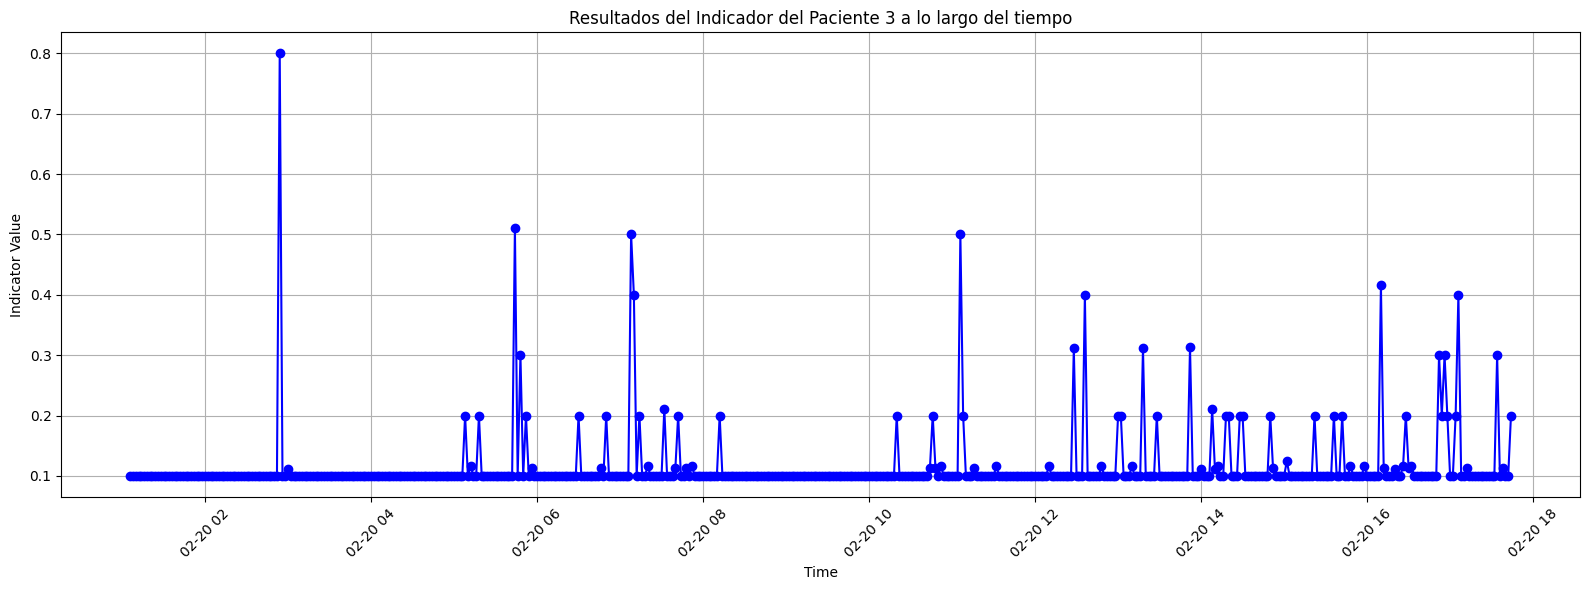
\includegraphics[width=\textwidth]{Images/indicador_de_criticidad_cambio.png}
  \caption{Evolución temporal del indicador de criticidad para el paciente 3. Se observa que durante los periodos de baja variabilidad y sin anomalías, el indicador permanece bajo, reflejando un estado fisiológico normal.}
  \label{fig:indicador_tiempo_paciente3}
\end{figure}

No obstante, esta suposición no es del todo correcta para pacientes que mantienen todos sus signos vitales consistentemente fuera del rango normal. De acuerdo al proceso de clasificación realizado, estos pacientes deberían clasificarse siempre en alto riesgo. Particularmente, ese es el caso del paciente 7, para el cual el modelo obtuvo un resultado pobre. La Figura \ref{fig:comparacion_clasificacion_paciente7} muestra la comparación entre el indicador de criticidad y la referencia objetiva para este paciente, evidenciando la discrepancia entre ambas clasificaciones. En este caso, el modelo subestima el riesgo al asumir que una baja variabilidad implica un estado de bajo riesgo, a pesar de que todos los signos vitales están fuera de rango.

\begin{figure}[H]
  \centering
  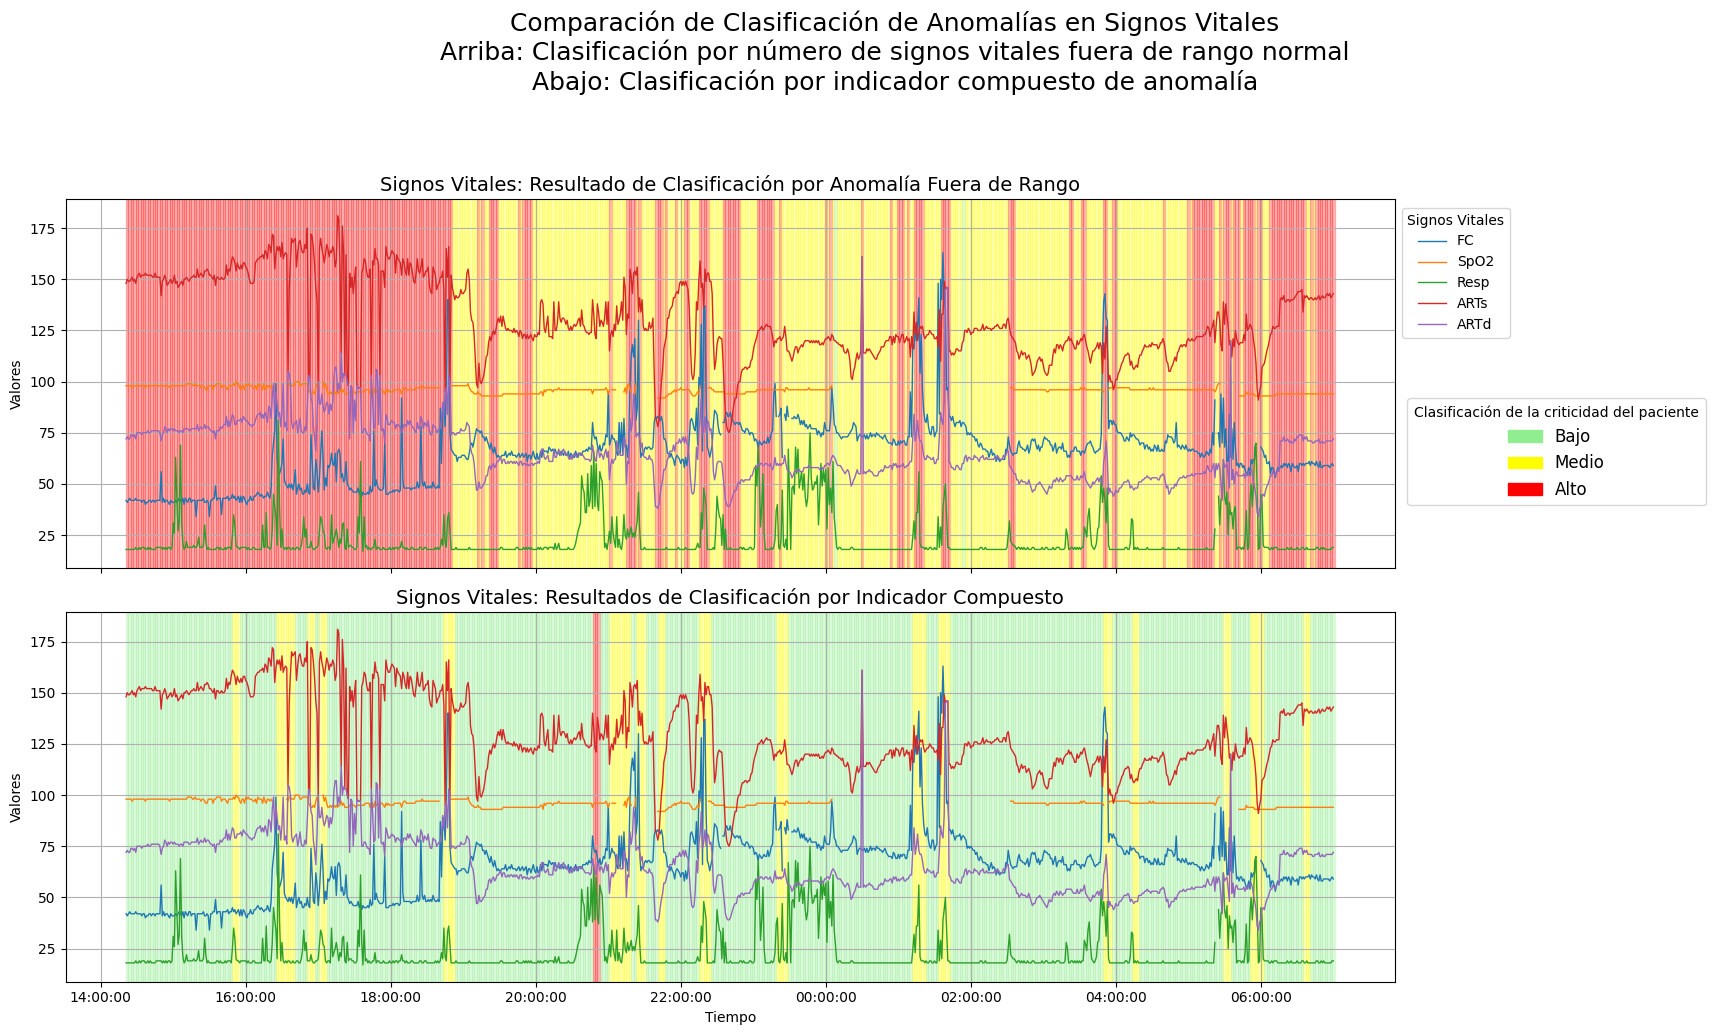
\includegraphics[width=\textwidth]{Images/comparacion_indicador_con_fuera_de_rango_paciente_7.png}
  \caption{Comparación de la clasificación de criticidad para el paciente 7: indicador de criticidad vs. número de signos vitales fuera de rango. El modelo subestima el riesgo al asumir que una baja variabilidad implica un estado de bajo riesgo, a pesar la mayoría de los signos vitales están fuera de rango.}

  \label{fig:comparacion_clasificacion_paciente7}
\end{figure}

Estos resultados resaltan la importancia de considerar el contexto clinico del paciente al interpretar los datos de signos vitales y al aplicar el modelos de detección de anomalías con el objetivo de clasificar correctamente su estado de salud. En particular, es fundamental reconocer que la baja variabilidad en los signos vitales no siempre indica un estado de bajo riesgo, especialmente en pacientes con condiciones crónicas o inestables. Por lo tanto, se sugiere que futuras investigaciones consideren incorporar información clínica adicional y ajustar el modelo para mejorar su capacidad de adaptación a diferentes perfiles de pacientes.

Para complementar el análisis cuantitativo, también se calcularon las métricas F1-Score y F2-Score, que proporcionan una medida más equilibrada entre precisión y recall. Estas métricas son especialmente útiles en contextos donde es importante minimizar tanto los falsos positivos como los falsos negativos. Los resultados de estas métricas se presentan en la última dos columnas de la Tabla \ref{tab:resultados_cuantitativos}, mostrando un rendimiento promedio del modelo en torno al 54\% para F1-Score y 55\% para F2-Score. Estos valores indican que, aunque el modelo logra una clasificación razonablemente precisa, aún existen oportunidades de mejora en su capacidad para identificar correctamente los estados de criticidad del paciente.

Adicionalmente, se realizó este mismo procedimiento de validación para el modelo de detección de anomalías anterior realizado por \cite{Vargas2023}, el cual se basa en la identificación de patrones anómalos en el espacio completo de las señales fisiológicas. Los resultados obtenidos para este modelo se presentan en la Tabla \ref{tab:resultados_cuantitativos_anterior}, permitiendo una comparación directa con el modelo basado en subespacios para el mismo conjunto de pacientes.

\begin{table}[H]
  \centering
  \resizebox{0.85\textwidth}{!}{%
    \begin{tabular}{
        >{\columncolor[HTML]{E8E8E8}}l
      llll}
      \cellcolor[HTML]{AFB8CC}Id                 & \cellcolor[HTML]{AFB8CC}Precisión & \cellcolor[HTML]{AFB8CC}Recall & \cellcolor[HTML]{AFB8CC}F1-Score & \cellcolor[HTML]{AFB8CC}F2-Score \\
      Paciente 1                                 & 0,67                              & 0,59                           & 0,51                             & 0,55                             \\
      Paciente 2                                 & 0,96                              & 0,08                           & 0,09                             & 0,06                             \\
      Paciente 3                                 & 0,99                              & 0,84                           & 0,91                             & 0,86                             \\
      Paciente 4                                 & 0,38                              & 0,33                           & 0,31                             & 0,30                             \\
      Paciente 5                                 & 0,85                              & 0,63                           & 0,72                             & 0,66                             \\
      Paciente 6                                 & 0,36                              & 0,15                           & 0,17                             & 0,15                             \\
      Paciente 7                                 & 0,66                              & 0,63                           & 0,63                             & 0,63                             \\
      \cellcolor[HTML]{D0D0D0}Resultado Promedio & 0,70                              & 0,46                           & 0,48                             & 0,46
    \end{tabular}
  }
  \caption{Resultados cuantitativos de la validación del modelo anterior basado en el análisis del espacio completo de las señales fisiológicas.}
  \label{tab:resultados_cuantitativos_anterior}
\end{table}

Al comparar directamente los resultados obtenidos para el F1-Score y F2-Score entre ambos modelos, se observa que el modelo basado en subespacios supera en promedio al modelo anterior, alcanzando un F1-Score promedio de 0,54 frente a 0,48 del modelo previo. Esto sugiere que el enfoque de subespacios es más efectivo para identificar correctamente el estado de criticidad del paciente. No obstante, es importante destacar que el modelo anterior presenta una precisión más alta en algunos pacientes, como el Paciente 1 y el Paciente 3, lo que indica que en ciertos casos específicos puede ser más adecuado. Sin embargo, en general, el modelo de subespacios demuestra una mayor robustez y adaptabilidad a diferentes perfiles de pacientes, lo que lo convierte en una opción preferible para la detección de anomalías en el contexto de monitoreo de signos vitales pediátricos.

\subsection{Resultados cualitativos}

Los resultados cualitativos de la validación del modelo de detección de anomalías en subespacios se centran en la utilidad clínica de las alertas generadas y su capacidad para proporcionar información relevante y accionable para los profesionales de la salud. Para evaluar esto, se realizó una revisión exhaustiva de las alertas generadas por el modelo y se compararon con las alertas producidas por el modelo anterior, que se basa en el análisis del espacio completo de las señales fisiológicas.

Para ilustrar estas diferencias, la Figura \ref{fig:alertas_modelo_anterior_paciente5} presenta los signos vitales del paciente 5, junto con los puntos marcados con diamantes rojos que indican los momentos en los que el modelo anterior reporta alertas debido a la detección de un estado anómalo. En este caso, aunque se identifican los periodos críticos relevantes (ya que coinciden en su mayoría con momentos con un mayor numero de signos vitales por fuer del rango normal), no es posible determinar a partir de la alerta cuáles señales específicas influyeron en su generación. Esta falta de información dificulta que el personal médico pueda reaccionar de manera precisa y dirigida, ya que no se sabe con claridad qué parámetros fisiológicos requieren mayor atención o intervención.

\begin{figure}[H]
  \centering
  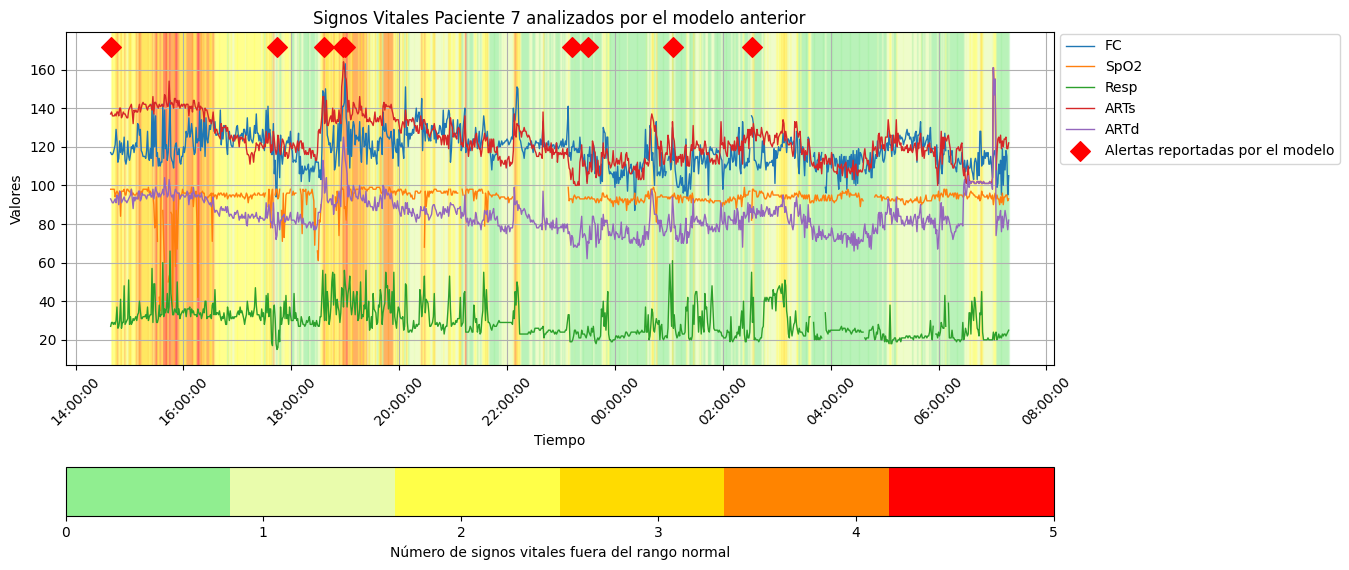
\includegraphics[width=\textwidth]{Images/alertas_modelo_anterior_paciente5.png}
  \caption{Signos vitales del paciente 5 con alertas (diamantes rojos) generadas por el modelo anterior basado en el análisis del espacio completo. La alerta no indica qué señales específicas contribuyeron al estado anómalo.}
  \label{fig:alertas_modelo_anterior_paciente5}
\end{figure}

En contraste, la Figura \ref{fig:alertas_subespacios_paciente5} muestra los signos vitales del mismo paciente, pero ahora resaltando las alertas generadas por el modelo de búsqueda en subespacios. En este diagrama, cada alerta está asociada explícitamente a una pareja de señales fisiológicas, correspondiente a aquella combinación que reporta mayor criticidad en ese instante. Esto permite identificar de manera clara cuáles parámetros están contribuyendo más significativamente al estado crítico del paciente. Gracias a esta información adicional, el personal médico puede comprender mejor el origen de la alerta y tomar decisiones más informadas y específicas sobre la intervención clínica necesaria.

\begin{figure}[H]
  \centering
  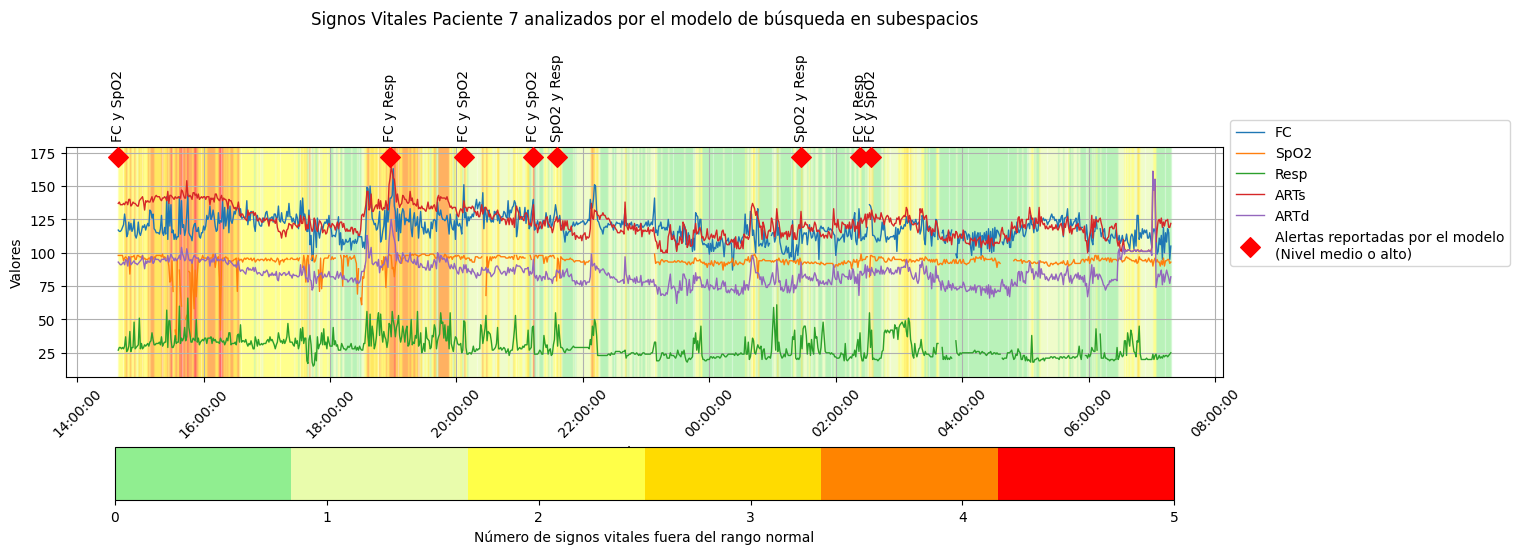
\includegraphics[width=\textwidth]{Images/alertas_subespacios_paciente5.png}
  \caption{Signos vitales del paciente 5 con alertas generadas por el modelo de búsqueda en subespacios. Cada alerta está asociada a una pareja de señales, lo que facilita identificar el origen de la criticidad y orientar la respuesta clínica.}
  \label{fig:alertas_subespacios_paciente5}
\end{figure}

Adicionalmente, el modelo propuesto permite evitar la generación de alertas poco relevantes en situaciones donde el paciente presenta todos sus signos vitales dentro del rango normal, gracias a la incorporación explícita de la edad del paciente en el proceso de detección de anomalías. Esta característica resulta especialmente relevante en el ámbito pediátrico, donde los rangos normales de los signos vitales varían considerablemente según la edad. Al considerar esta variable, el modelo es capaz de filtrar alertas que no aportan información clínica significativa, evitando así notificaciones innecesarias como las que fueron reportadas por el modelo anterior entre las 22:00 y las 24:00 horas del paciente 5, periodo en el cual todos los signos vitales se encontraban dentro de los límites normales para su edad (véase Figura~\ref{fig:alertas_modelo_anterior_paciente5}). En estos casos, el modelo de subespacios no genera alertas superfluas, lo que contribuye a reducir la sobrecarga de alarmas y permite al personal médico enfocar su atención en situaciones realmente críticas.

Para validar este resultado entre todos los pacientes, se realizó un análisis respecto a la generación de falsas alertas, es decir, aquellas alertas que se generan cuando el paciente no presenta signos vitales fuera del rango normal. La Tabla \ref{tab:resultados_cualitativos} resume los resultados de este análisis para cada paciente, indicando el número total de alertas generadas por el modelo de subespacios y cuántas de ellas corresponden a situaciones donde todos los signos vitales están dentro del rango normal.

\begin{table}[H]
  \centering
  \resizebox{0.95\textwidth}{!}{%
    \begin{tabular}{
        >{\columncolor[HTML]{E8E8E8}}l
        >{\raggedright\arraybackslash}p{6cm}
      >{\raggedright\arraybackslash}p{6cm}}
      \cellcolor[HTML]{AFB8CC}Id
      & \cellcolor[HTML]{AFB8CC}Instantes con falsas alertas reportadas por el modelo de búsqueda en subespacios
      & \cellcolor[HTML]{AFB8CC}Instantes con falsas alertas reportadas por el modelo original \\
      Paciente 1                              & 91                                                                                                     & 267                                                                                  \\
      Paciente 2                              & 485                                                                                                    & 481                                                                                  \\
      Paciente 3                              & 85                                                                                                     & 408                                                                                  \\
      Paciente 4                              & 15                                                                                                     & 17                                                                                   \\
      Paciente 5                              & 228                                                                                                    & 31                                                                                   \\
      Paciente 6                              & 110                                                                                                    & 271                                                                                  \\
      Paciente 7                              & 52                                                                                                     & 263                                                                                  \\
      \cellcolor[HTML]{D0D0D0}Resultado Total & 1066                                                                                                   & 1738                                                                                 \\
    \end{tabular}
  }
  \caption{Comparación del número de instantes con falsas alertas generadas por el modelo de búsqueda en subespacios y el modelo original para cada paciente.}
  \label{tab:resultados_cualitativos}
\end{table}

Los resultados muestran que el modelo de subespacios genera significativamente menos falsas alertas en comparación con el modelo original. En total, se reportaron 1066 instantes con falsas alertas por parte del modelo de subespacios, mientras que el modelo original generó 1738 instantes de falsas alertas. Esto representa una reducción del 38,7\% en la cantidad de alertas innecesarias, lo cual es un resultado significativo considerando la importancia de minimizar la sobrecarga de alarmas en entornos clínicos.

En general, los resultados cualitativos indican que el modelo de búsqueda en subespacios no solo mejora la precisión en la detección de anomalías, sino que también proporciona alertas más útiles y relevantes para el personal médico. Al asociar cada alerta a una pareja específica de señales fisiológicas, se facilita la identificación de patrones críticos y se optimiza la respuesta clínica, contribuyendo así a una atención más efectiva y centrada en el paciente. Por otra parte, la reducción de falsas alertas permite mejorar la confianza del personal médico en el sistema de monitoreo, al disminuir la cantidad de notificaciones irrelevantes que pueden generar distracción o fatiga ante alarmas.

\section{Código de validación}

A continuación se presenta el código utilizado para realizar la validación del modelo de detección de anomalías en subespacios, incluyendo la categorización de los datos y el cálculo de las métricas de precisión, exactitud, F1-Score y F2-Score. Este código utiliza las librerías \textit{pandas} y \textit{sklearn.metrics} de Python para procesar los datos y calcular las métricas de validación.

\begin{minted}[fontsize=\small, linenos, breaklines]{python}
import pandas as pd
from sklearn.metrics import classification_report, f1_score, fbeta_score

# El DataFrame patient_data contiene, para cada instante de tiempo, la columna 'Normalized Vitals', que representa la cantidad de signos vitales fuera de su rango normal, dividida por el número total de signos vitales disponibles para ese paciente. De esta manera, el valor está normalizado entre 0 y 1, indicando la proporción de signos vitales alterados en cada momento.

# Por otro lado, el DataFrame indicator_data incluye la columna 'Normalized Indicator', que corresponde al valor del indicador de criticidad en cada instante, normalizado por el número de subespacios disponibles en ese momento. Así, este valor también se encuentra entre 0 y 1 y permite comparar la criticidad detectada por el modelo con la proporción de signos vitales alterados.

def categorize_vitals_and_indicator(patient_data, indicator_data):
    """
    Categoriza los valores normalizados del indicador de criticidad y del numero de signos vitales fuera de rango en tres categorías: bajo, medio y alto, según umbrales definidos.
    """
    low_th = 0.3
    high_th = 0.6

    # Categoría para anomalías normalizadas
    patient_data['True Category'] = pd.cut(
        patient_data['Normalized Vitals'],
        bins=[-float('inf'), low_th, high_th, float('inf')],
        labels=['Low', 'Medium', 'High']
    )

    # Categoría para el indicador
    indicator_data['Indicator Category'] = pd.cut(
        indicator_data['Normalized Indicator'],
        bins=[-float('inf'), low_th, high_th, float('inf')],
        labels=['Low', 'Medium', 'High']
    )

    # Sincroniza ambos DataFrames
    comparison_df = pd.DataFrame({
        'Start Time': indicator_data['Start Time'].values,
        'End Time': indicator_data['End Time'].values,
        'True Category': patient_data['True Category'].values,
        'Indicator Category': indicator_data['Indicator Category'].values
      })

    return comparison_df

def calculate_metrics(comparison_df):
    """
    Calcula precisión, recall, F1 y F2-score usando sklearn.metrics.
    """
    report = classification_report(
        comparison_df['True Category'],
        comparison_df['Indicator Category'],
        output_dict=True,
        zero_division=0
    )
    f1 = f1_score(comparison_df['True Category'], comparison_df['Indicator Category'], average='weighted')
    f2 = fbeta_score(comparison_df['True Category'], comparison_df['Indicator Category'], beta=2, average='weighted')

    return report['weighted avg']['precision'], report['weighted avg']['recall'], f1, f2

def count_false_positives(comparison_df)
   """
    Cuenta los falsos positivos: instantes donde el indicador predice anomalía pero no hay anomalía real.
    """
    return ((comparison_df[indicator_col] != 'Low') & (comparison_df['True Category'] == 'Low')).sum()

# Calcula las métricas de validación
comparison_df = categorize_vitals_and_indicator(patient_data, indicator_data)
precision, recall, f1, f2 = calculate_metrics(comparison_df)
false_positives = count_false_positives(comparison_df)
\end{minted}